% !TeX root=../main.tex

\chapter{مقدمه}
% دستور زیر باعث عدم‌نمایش شماره صفحه در اولین صفحهٔ این فصل می‌شود.
%\thispagestyle{empty}
\section{آشنایی با این راهنما}
حروف‌چینی پروژه کارشناسی، پایان‌نامه یا رساله یکی از موارد پرکاربرد استفاده از
\lr{\LaTeX}
و زی‌پرشین
\cite{Khalighi87xepersian}
است. یک پروژه، پایان‌نامه یا رساله، احتیاج به تنظیمات زیادی از نظر صفحه‌آرایی دارد که وقت زیادی از دانشجو می‌گیرد. به دلیل قابلیت‌های بسیار لاتک در حروف‌چینی، کلاسی با نام 
\lr{tehran-thesis}
برای حروف‌چینی پروژه‌ها، پایان‌نامه‌ها و رساله‌های دانشگاه تهران، بر مبنای کلاس مشابه
\lr{IUST-Thesis}
تهیه شده است. این کلاس و فایل‌های همراه آن به گونه‌ای طراحی شده است که مطابق با دستورالعمل نگارش و تدوین پایان‌نامه کارشناسی ارشد و دکتری پردیس دانشکده‌های فنی دانشگاه تهران
\cite{UTThesisGuide}
باشد.

دستورالعمل نگارش و تدوین پایان‌نامه دانشگاه تهران به دو مقوله می‌پردازد، اول قالب و چگونگی صفحه‌آرایی پایان‌نامه، مانند اندازه و نوع قلم بخشهای مختلف، چینش فصلها، قالب مراجع و مواردی از این قبیل و دوم محتوای هر فصل پایان‌نامه. 
درصورت استفاده از این کلاس، نیازی نیست که دانشجو نگران مقوله اول باشد و پس از تایپ مطالب خود می‌تواند آنها را با لاتک و ابزار آن اجرا کند تا پایان‌نامه خود را با قالب دانشگاه داشته باشد. همچنین با خواندن این راهنما از ملزومات محتوایی هر فصل پایان‌نامه نیز مطلع خواهد شد.

در ادامهٔ  مقدمهٔ این راهنما، ابتدا چگونگی استفاده از کلاس پایان‌نامه و فایل‌های همراه آن را به صورت فنی شرح می‌دهیم و سپس مطالبی را در مورد ویژگی‌های محتوایی فصل ۱ پایان‌نامه (یعنی مقدمه) خواهیم آورد.
بقیهٔ فصل‌های این راهنما، تنها خصوصیات محتوایی فصول مختلف پایان‌نامه را شرح خواهند داد. نهایتاً جهت یادآوری، در پیوست‌ها مطالبی دربارهٔ آشنایی با دستورات لاتک، مدیریت مراجع در لاتک و چگونگی رسم جداول، نمودارها و الگوریتم‌ها آورده خواهند شد.

\section{چگونگی استفاده از کلاس پایان‌نامه}
کلیه فایل‌های لازم برای حروف‌چینی با کلاس فوق، داخل پوشه‌ای به نام
\lr{tehran-thesis}
قرار داده شده است. توجه داشته باشید که برای استفاده از این کلاس باید فونت‌های
\lr{IRLotusICEE}
و
\lr{IRTitr}
را داشته باشید (که همراه با این کلاس هست و نیاز به نصب نیست).
قلم‌های
\lr{IRLotusICEE}
مستخرج از قلم‌های استاندارد
\lr{IRLotus}
شورای عالی اطلاع‌رسانی%
\footnote{
قلم‌های استاندارد
\lr{IRFonts}
از شورای عالی اطلاع‌رسانی، منطبق بر آخرین نسخه استاندارد یونیکد، استاندارد ملی ۶۲۱۹ و استاندارد
\lr{Adobe Glyph Naming}
هستند.
}
هستند که توسط دکتر بابایی‌زاده اصلاحاتی روی آنها صورت پذیرفته است: تبدیل صفر توپر به صفر توخالی (جهت تمایز بیشتر با نقطه) و اضافه شدن
\textit{\textbf{حالت توپر و ایرانیک توأم}}،
که این موارد در قلم‌های شورای عالی اطلاع‌رسانی وجود ندارد.

\subsection{این همه فایل؟!}
\label{muchFiles}
از آنجایی که یک پایان‌نامه یا رساله، یک نوشته بلند محسوب می‌شود، لذا اگر همه تنظیمات و مطالب پایان‌نامه را داخل یک فایل قرار بدهیم، باعث شلوغی و سردرگمی می‌شود. به همین خاطر، قسمت‌های مختلف پایان‌نامه یا رساله  داخل فایل‌های جداگانه قرار گرفته است. مثلاً تنظیمات پایه‌ای کلاس داخل فایل
\lr{tehran-thesis.cls}، 
قسمت مشخصات فارسی پایان‌نامه داخل 
\lr{faTitle.tex}،
مطالب فصل اول داخل 
\lr{chapter1.tex}
و تنظیمات قابل تغییر توسط کاربر داخل 
\lr{commands.tex}،
قرار داده شده است.
\textbf{
	فایل اصلی این مجموعه، فایل
	\lr{main.tex}
	می‌باشد.
}
% یعنی بعد از تغییر فایل‌های دیگر، برای دیدن نتیجه تغییرات، باید این فایل را اجرا کرد. بقیه فایل‌ها به این فایل، کمک می‌کنند تا بتوانیم خروجی کار را ببینیم.
اگر به فایل 
\lr{main.tex}
دقت کنید، متوجه می‌شوید که قسمت‌های مختلف پایان‌نامه، توسط دستورهایی مانند 
\lr{input}
و
\lr{include}
به فایل اصلی، یعنی 
\lr{main.tex}
معرفی شده‌اند.
با توجه به ساختار محتوایی دستورالعمل، در فایل
\lr{main.tex}
فرض شده که پایان‌نامه یا رساله شما، از ۵ فصل و تعدادی پیوست تشکیل شده است. با اینحال، شما می‌توانید به راحتی فصل‌ها و پیوست‌ها را با صلاحدید اساتید راهنما، کم و زیاد کنید. این کار، بسیار ساده است. فرض کنید بخواهید یک فصل دیگر هم به پایان‌نامه اضافه کنید. برای این کار، کافی است یک فایل با نام دلخواه مثلاً 
\lr{chapter6}
و با پسوند 
\lr{.tex}
بسازید و آن را داخل پوشه 
\lr{tehran-thesis}
قرار دهید و سپس این فایل را با دستور 
\verb!\include{chapter6}!
داخل فایل
\lr{main.tex}
 فراخوانی کنید.

\subsection{از کجا شروع کنم؟}
قبل از هر چیز، باید یک توزیع تِک مناسب مانند تک‌لایو
\lr{(TeXLive)}
را روی سیستم خود نصب کنید. تک‌لایو  را می‌توانید از 
 \href{http://www.tug.org/texlive}{سایت رسمی آن}%
\LTRfootnote{\lr{\url{http://www.tug.org/texlive}}}
 دانلود کنید یا مستقیماً از مخازن توزیع لینوکس خود بگیرید (مثلاً در اوبونتو با دستور
\LRE{\verb!sudo apt install texlive-full!}).
برای نصب تک‌لایو و اجرای اسناد زی‌پرشین می‌توانید از
\href{http://parsilatex.com/site/shop/}{دی‌وی‌دی مجموعه پارسی‌لاتک}%
\LTRfootnote{\lr{\url{http://parsilatex.com/site/shop/}}}
و فایل راهنمای موجود در آن هم کمک بگیرید.

برای تایپ و پردازش اسناد لاتک باید از یک ویرایشگر مناسب استفاده کنید. ویرایشگرهای
\lr{TeXWroks},
\lr{TeXstudio},
\lr{Texmaker}
و
\lr{BiDiTeXmaker}
بدین منظور تولید شده‌اند. می‌توان ویرایش‌گر 
 \href{https://bitbucket.org/srazi/biditexmaker3}{\lr{BiDiTeXmaker}}%
 \LTRfootnote{\lr{\url{https://bitbucket.org/srazi/biditexmaker3}}}
را که بویژه برای کار با زی‌پرشین و مطالب دوجهته بهبود یافته است، بهینه‌ترین ویرایشگر لاتک برای کار با اسناد فارسی عنوان کرد.
 
حال اگر نوشتن \پ اولین تجربه شما از کار با لاتک است، توصیه می‌شود که یک‌بار به صورت اجمالی، کتاب «%
\href{http://www.tug.ctan.org/tex-archive/info/lshort/persian/lshort.pdf}{مقدمه‌ای نه چندان کوتاه بر
\lr{\LaTeXe}}%
\LTRfootnote{\lr{\url{http://www.tug.ctan.org/tex-archive/info/lshort/persian/lshort.pdf}\hfill}}»
ترجمه دکتر مهدی امیدعلی را مطالعه کنید. این کتاب، کتاب بسیار کاملی است که خیلی از نیازهای شما در ارتباط با حروف‌چینی را برطرف می‌کند.
اگر تک لایو کامل را داشته باشید، این کتاب را هم دارید. کافیست در خط فرمان دستور زیر را بزنید:
\begin{latin}
	\texttt{texdoc lshort-persian}
\end{latin}
اگر عجله دارید، برخی دستورات پایه‌ای مورد نیاز در پیوست \ref{app:latexIntro} بیان شده‌اند.
 
بعد از موارد گفته شده، فایل 
\lr{main.tex}
و
\lr{faTitle.tex}
را باز کنید و مشخصات پایان‌نامه خود مثل نام، نام خانوادگی، عنوان پایان‌نامه و ... را جایگزین مشخصات موجود در فایل
\lr{faTitle.tex}
 کنید. نیازی نیست نگران چینش این مشخصات در فایل پی‌دی‌اف خروجی باشید، زیرا کلاس 
\lr{tehran-thesis}
همه این کارها را بطور خودکار برای شما انجام می‌دهد. در ضمن، موقع تغییر دادن دستورهای داخل فایل
\lr{faTitle.tex}
 کاملاً دقت کنید؛ این دستورها، خیلی حساس هستند و ممکن است با یک تغییر کوچک، موقع اجرا، خطا بگیرید. برای دیدن خروجی کار، فایل 
\lr{faTitle.tex}
 را 
\lr{Save}
(نه 
\lr{Save As})
کنید و بعد به فایل 
\lr{main.tex}
برگشته و آن را اجرا کنید%
\footnote{
	البته فایلهای این مجموعه به گونه‌ای هستند که در
	\lr{TeXWorks} یا
	\lr{TeXstudio}
	بدون بازگشت به فایل اصلی، می‌توانید سند خود را اجرا کنید.
}.
 حال اگر می‌خواهید مشخصات انگلیسی \پ را هم عوض کنید، فایل 
\lr{enTitle.tex}
را باز کنید و مشخصات داخلش را تغییر دهید.
%\RTLfootnote{
%برای نوشتن پروژه کارشناسی، نیازی به وارد کردن مشخصات انگلیسی پروژه نیست. بنابراین، این مشخصات بطور خودکار، نادیده گرفته می‌شود.
%}
در اینجا هم برای دیدن خروجی باید این فایل را ذخیره کرده، بعد به فایل 
\lr{main.tex}
برگشته و آن را اجرا کرد.

برای راحتی بیشتر، کلاس 
\lr{tehran-thesis.cls}
طوری طراحی شده است که کافی است فقط  یک‌بار مشخصات \پ را (در فایل‌های
\lr{faTitle.tex}
و
\lr{enTitle.tex})
وارد کنید و هر جای دیگر که این مشخصات لازم باشند، به طور خودکار درج می‌شوند. با این حال، اگر مایل بودید، می‌توانید تنظیمات موجود را تغییر دهید؛ گرچه، در صورتیکه کاربر مبتدی هستید و یا با ساختار فایل‌های  
\lr{cls}
 آشنایی ندارید، بهتر است به فایل 
\lr{tehran-thesis.cls}
دست نزنید.

نکته دیگری که باید به آن توجه کنید این است که در قالب آماده شده، سه گزینه به نام‌های
\lr{bsc}،
\lr{msc}
و
\lr{phd}
برای نوشتن پروژه، پایان‌نامه و رساله، در نظر گرفته شده است. بنابراین اگر قصد تایپ پروژهٔ کارشناسی، پایان‌نامهٔ کارشناسی ارشد یا رسالهٔ دکتری را دارید، به ترتیب باید از گزینه‌های
\lr{bsc}،
\lr{msc}
و
\lr{phd}
در فایل 
\lr{main.tex}
استفاده کنید. با انتخاب هر کدام از این گزینه‌ها، تنظیمات مربوط به آنها به طور خودکار، اعمال می‌شود.


\subsection[مطالب پایان‌نامه را چطور بنویسم؟]
{مطالب \پ را چطور بنویسم؟}
\subsubsection{نوشتن فصل‌ها}
همان‌طور که در بخش \ref{muchFiles} گفته شد برای جلوگیری از شلوغی، قسمت‌های مختلف \پ از جمله فصل‌ها، در فایل‌های جداگانه‌ای قرار داده شده‌اند. 
مثلاً اگر می‌خواهید مطالب فصل ۱ را تایپ کنید، باید فایل‌های 
\lr{main.tex}
و
\lr{chapter1.tex}
را باز کرده و مطالب خود را جایگزین محتویات داخل 
\lr{chapter1.tex}
نمایید. دقت شود که در ابتدای برخی فایلها دستوراتی نوشته شده است و از شما خواسته شده که آن دستورات را حذف نکنید.

%توجه کنید که همان‌طور که قبلاً هم گفته شد، تنها فایل قابل اجرا، 
%\lr{main.tex}
%است. لذا برای دیدن حاصل (خروجی) فایل خود، باید  
%\lr{chapter1.tex}
%را ذخیره کرده و سپس فایل 
%\lr{main.tex}
%را اجرا کنید.

نکته بسیار مهمی که در اینجا باید گفته شود این است که سیستم \lr{\TeX}، محتویات یک فایل تِک را به ترتیب پردازش می‌کند.  بنابراین، اگر مثلاً  دو فصل اول خود را نوشته و خروجی آنها را دیده‌اید و مشغول تایپ مطالب فصل ۳ هستید، بهتر است
که دو دستور 
\verb!% !TeX root=../main.tex

\chapter{مقدمه}
% دستور زیر باعث عدم‌نمایش شماره صفحه در اولین صفحهٔ این فصل می‌شود.
%\thispagestyle{empty}
\section{معرفی ویژگی‌های متمایزکننده‌ی شبکه‌ی اینترنت اشیا}
رشد شبکه های اینترنت اشیا کاربردهای زیادی از جمله سیستم پایش سلامت \footnote{\lr{health-care system}}،‌ خانه‌ی هوشمند \footnote{smart home} و شهر هوشمند \footnote{smart city}را توسعه بخشیده است. بخش زیربنایی کاربردهای مبتنی بر شبکه‌های اینترنت اشیا، اندازه‌گیری و گزارش دیتاهایی مانند دما، رطوبت، ویدیو و ... می‌باشد. این اطلاعات از طریق درگاه‌\footnote{gateway}ها به گره‌های مصرف کننده می‌رسد. افزایش تعداد گره‌های مصرف کننده و نیز تعداد حسگرها ترافیک عظیمی در شبکه‌های اینترنت اشیا را ایجا کرده و نیز میزان تراکم در این شبکه‌ها را بالا می‌برد. این مسئله باعث کاهش میزان کیفیت سرویس می‌شود. به علاوه اینکه فعالسازی دوباره‌ی حسگرها برای واکشی پاسخ، میزان انرژی مصرفی آنها را بالا برده و از عمر باتری آنها کم می‌کند.

شبکه‌های اینترنت اشیا دارای دو ویژگی متمایز و چالش‌زا می‌باشند. اول اینکه تأمین انرژی اکثر تجهیزات و حسگرها از طریق باتری تأمین می‌شود و بنابراین با انرژی محدود کار می‌کنند و بالا بودن حچم درخواست‌ها باعث می‌شود تا از دست دادن انرژی در آنها سریعتر رخ دهد. دوم اینکه دیتای گزارش شده توسط حسگرها برای مدت زمان کوتاهی معتبر یا به عبارتی تازه می‌باشد و پس از مدتی منقضی می‌شود. در بعضی از مقالات به ویژگی دوم تحت عنوان تازگی دیتا\footnote{\lr{data freshness}} و در بعضی دیگر تحت یک مفهوم کلی تر با نام سن اطلاعات\footnote{\lr{Age of Information (AoI)}} اشاره شده است. 
\subsection{استراتژی ذخیره‌سازی}
حال ذخیره سازی به عنوان راه حلی برای متوازن‌سازی ترافیک در شبکه مطرح می‌شود به این معنا که در درگاه‌های شبکه‌های اینترنت اشیا یک حافظه‌ی ذخیره‌سازی قرار گرفته است که اطلاعات را جمع‌آوری می‌کند و می‌تواند به طور موقت دیتا را ذخیره کرده و در صورت ارسال درخواست از سوی گره‌های مصرف کننده، دیتای مربوطه را برای آنها بفرستد. 

در سناریوی توصیف شده از ارتباط مستقیم لینک‌های پشتی\footnote{\lr{backhaul links}} با حسگرها جلوگیری کرده‌ایم که در اثر آن ترافیک شبکه معادلتر شده و حجم درخواست‌های ارسالی به یک حسگر کاهش می‌یابد و بنابراین حسگر به تعداد دفعات کمتری برای واکشی پاسخ فعال می‌شود و مصرف انرژی در آن کاهش‌ می‌یابد. در سناریوی مطرح شده باید قیدی را مبنی بر محدودیت حافظه‌ی ذخیره‌سازی در نظر داشته باشیم به علاوه‌ی اینکه به طراحی یک سیاست مناسب برای ذخیره‌سازی محتوا با در نظر گرفتن فاکتور تازگی دیتا نیاز داریم.  

تعداد قابل توجهی از تحقیقات تا قبل از سال 2018 به یک استراتژی ذخیره‌سازی مبتنی بر محتوا\footnote{\lr{ICN caching}} برای یک نیاز خاص در شبکه‌های اینترنت اشیا پرداخته‌اند و روش‌هایی را مبتنی بر طبیعت \lr{ad-hoc} و بی‌سیم شبکه‌های اینترنت اشیا ارائه کرده‌اند. 

عموماً یک استراتژی ذخیره‌سازی می‌تواند بر دو جنبه اثر بگذارد: یکی اینکه کدام محتوا در حافظه‌ی کش ذخیره گردد که به عبارتی به تصمیم برای ذخیره‌ی محتوا\footnote{\lr{caching decision}} می‌پردازد و دیگری آنکه در صورتیکه ظرفیت حافظه‌ی کش پر شود، الویت با حذف کدام یک از محتواها می‌باشد و یا به عبارتی مکانیزم یا سیاست جایگزینی محتوا\footnote{\lr{cache replacement policy}} را تحت تأثیر قرار می‌دهد. 

\subsubsection{\lr{LCE(Leave Copy Everywhere)}}
سر راست ترین استراتژی ذخیره‌سازی \lr{CEE} یا به تعبیری \lr{LCE (Leave Copy Everywhere)} می‌باشد. در این حالت تمامی گره‌های مسیر برای ذخیره‌سازی محتوای ورودی تلاش می‌کنند. در شبکه‌های مرسوم مبتنی بر محتوا، با توجه به این موضوع که به طور پیش‌فرض محتوا حجم زیادی دارد، این روش با اغماض قابل قبول بوده و سربار کمی نیز ایجاد می‌کند و برتری اصلی آن در اینست که سریعترین انتشار ممکن از محتوا را پیشنهاد می‌دهد.

در این استراتژی گره‌های مسیر هر محتوایی را که شنود می‌کنند، بلافاصله در حافظه ذخیره می‌نمایند. این مسئله وجود کپی از محتوا را تضمین می‌نماید ولی باعث می‌شود تا بیش از حد مورد نیاز کپی از آن محتوا وجود داشته باشد در حالیکه از قابلیت‌ها و منابع شبکه به درستی استفاده نکرده‌ایم. عملاً یکی از اهداف در این مسئله کاهش موارد زائد و بالا بردن تنوع می‌باشد یعنی انتظار داریم تا در حافظه‌های مختلف، چینش‌های متفاوتی از محتواهای موجود ذخیره شده باشند. 
\subsubsection{\lr{ProbCache caching}}
دو پیاده‌سازی استاتیک و دینامیک برای این استراتژی ذخیره‌سازی وجود دارد. در استراتژی استاتیک، یک مقدار ثابت \lr{p} و بتبع بین 0 و 1 برای احتمال ذخیره سازی در گره‌های مسیر درنظر گرفته می‌شود. با گذر محتوای جدید از هر گره در مسیر، آن گره یک عدد رندوم تولید کرده و در صورتیکه این مقدار از \lr{p} کمتر باشد، محتوا را ذخیره می‌کند و در غیر اینصورت آن را تنها جلو می‌راند. 

در این شرایط محتوای محبوب تر که در طول زمان با نرخ بیشتری درخواست می‌شود،‌ شانس بالاتری برای ذخیره سازی پیدا می‌کند. در واقع احتمال ذخیره‌سازی محتوا بعد از \lr{n} بار دریافت شدن به صورت $1-(1-p)^n$ محاسبه می‌شود که با افزایش \lr{n} این مقدار به 1 میل می‌کند. یعنی هر چه میزان محبوبیت فایل یا محتوا بیشتر باشد، احتمال ذخیره‌ی آن نیز افزایش می‌یابد. 

در حالت دینامیک احتمال ذخیره کردن محتوا در یک گره براساس پارامترهایی مانند تازگی،‌ نوع یا تولیدکننده‌ی محتوا، میزان سطح انرژی گره، توپولوژی شبکه و گره های مجاور آن و یا سایر اطلاعات محلی ایجاد می‌گردد.

\subsubsection{\lr{Betweenness Centrality Caching}}
در این استراتژی پارامتری براساس توپولوژی شبکه برای هر گره محاسبه می‌شود. درواقع تعداد بارهایی که آن گره در مسیرهایی بین فرستده و گیرنده قرار می‌گیرد، محاسبه شده و بسته به توپولوژی در جایی که این پارامتر بیشینه می گردد،‌ یک کپی از محتوا ذخیره می‌شود.

\subsubsection{\lr{LCD(Leave Copy Down)}}
در این استراتژی ذخیره‌سازی یک کپی و آن هم در نزدیکترین گره به سنسور، یعنی در درگاه متصل به سنسور قرار داده می‌شود. در این حالت کپی‌های زائد از محتوای مدنظر در سایر گره‌ها قرار ندارد، درواقع نسبت به حالت‌های قبلی از این حیٍث استفاده‌ی بهینه‌تری از منابع کرده‌ایم اما همچنان برای واکش پاسخ، درخواست ارسال شده تا گره یکی مانده به سنسور بالا می‌رود که این مسئله چندان مطلوب نیست.

\subsubsection{\lr{Edge Caching}}
در استراتژی ذخیره‌سازی لبه مانند حالت \lr{LCD} یک کپی از محتوا ولی دقیقاً در خلاف جهت آن یعنی در نزدیکترین گره به مصرف کننده یا در دستگاه کاربر ذخیره می‌گردد که عملا مشکل حالت قبلی در اینجا رفع شده است یعنی درخواست برای واکشی پاسخ تا حسگر یا گره‌های نزدیک به آن بالا نمی‌رود و عملاً از جحم ترافیک شبکه کم می‌شود.

\paragraph{}
در شکل \ref{fig:cachingStrategy} استراتژی‌های متداول در شبکه‌های مبتنی بر محتوا را (که پیشتر به آنها اشاره شد،) مشاهده می‌کنید.
\begin{figure}[ht]
	\centerline{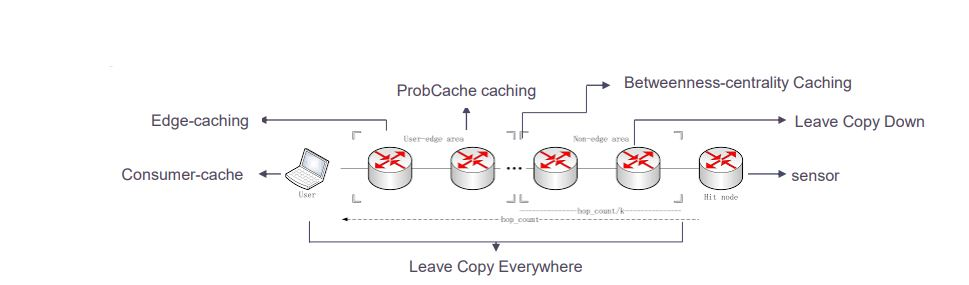
\includegraphics[width=13cm]{cachingStrategy}}
	\caption{استراتژی های متداول ذخیره‌سازی در شبکه‌های مبتنی بر محتوا برگرفته از\\ \lr{\href{https://mdpi-res.com/d_attachment/futureinternet/}{future internet}}}
	\label{fig:cachingStrategy}
\end{figure}

\subsection{سیاست جایگزینی محتوا}
در عمل به دلیل سایز محدود حافظه‌ی ذخیره‌سازی به یک سیاست مناسب برای جایگزینی محتوا در حافظه نیاز داریم. درواقع اصلی ترین هدف ما، یافتن بهینه ترین سیاست در تعامل با محیط می‌باشد به گونه‌ای که میزان تأخیر در ارسال دیتا برای یک محتوا را کمینه نماید.

  قطعاً استراتژی ذخیره‌سازی برای بعضی از محتویات که در طول زمان هیچ درخواستی برای آنها در شبکه وجود ندارد‌ و قبل از انتظار ما برای برآوردن درخواست دیتای مربوط به آنها منقضی می‌شود، مطلوب ما نیست. به عبارتی می توان گفت که در این حالت یک سیاست جایگزینی محتوای مناسب به کارایی استراتژی ذخیره‌‌سازی انتخاب شده، ‌کمک خواهد کرد. یک سری روش رایج برای شبکه‌های \lr{NDN} تعریف گردیده است که برجسته‌ترین و قدیمی‌ترین سیاست مطرح شده، \lr{FIFO (First Input, First Output)} می‌باشد.
  
  سیاست‌های جایگزینی مرسوم،‌ به چهار دسته مطابق با جدول\eqref{tab:replacementPolicies} تقسیم می‌گردند که در ادامه به آنها می‌پردازیم.
  \begin{table}[ht]
  	\caption{سیاست‌های مرسوم برای جایگزینی محتوا}
  	\label{tab:replacementPolicies}
  	\centering
  	\onehalfspacing
  	\begin{tabular}{|r|c|l|r|}
  		\hline \lr{Existing Plicies} & \lr{Description} & \lr{Category} \\ 
  		\hline \lr{LRU, LRU-threshold,} & \lr{Keeps the recently referenced objects} & \lr{Recency-based} \\
  			   \lr{LRU-hot, SLRU,} & \lr{} & \lr{} \\ 
  			   \lr{HLRU, LRU-LSC} & \lr{} & \lr{} \\ 
  		\hline \lr{LFU, LFU-Aging,} & \lr{Keeps the most requested objects} & \lr{Frequency-based} \\ 
  			\lr{LFU-DA, swLFU} & \lr{} & \lr{} \\
  		\hline \lr{RR, RAND,} & \lr{A simple random choice} & \lr{Randomized Policies} \\ 
  		\lr{HARMONIC} & \lr{to avoid computation overhead} & \lr{} \\
  		\hline \lr{SIZE, PSS, CSS} & \lr{Evicts large contents} & \lr{Size-based} \\ 
  		\hline 
  	\end{tabular} 
  \end{table}
  
  \subsubsection{\lr{Recency-Based Replacement Policies}}
  معروف‌‌ترین و پرکاربردترین سیاست از میان سیاست‌های جایگزینی محتوا در این دسته، سیاست \lr{LRU(Least Recently Used)} می‌باشد. (می توان گفت که سایر سیاست‌های متعلق به این دسته از سیاست \lr{LRU} مشتق شده‌اند.) در این حالت هریک از گره‌ها مجموعه‌ی درخواست‌های ارسال شده برای هریک از محتوا را دنبال می‌کند و زمانیکه نیاز به جایگزینی محتوا برای ذخیره‌ی محتوای جدید باشد، محتوایی را که اخبراً از آن کمتر از سایرین استفاده شده است را از حافظه دور می‌ریزد و فایل جدید را ذخیره می‌کند. روش مطرح شده نسبت به سایر سیاست‌های جایگزینی، کارایی بسیار بالایی دارد، اما در شرایطی که تعداد محتویات محبوب از سایز حافظه بیشتر باشد، شبکه دچار اختلال\footnote{\lr{thrashing}} خواهد شد.
  
  \subsubsection{\lr{Frequency-Based Replacement Policies}}
  سیاست اصلی در این گروه، سیاست \lr{LFU(Least Frequency Used)} می‌باشد. در واقع برخلاف سیاست \lr{LRU} که به سوال درباره‌ی آخرین بار استفاده از محتوا پاسخ می‌دهد،  سیاست \lr{LFU} میزان درخواست برای دیتای محتوا را دنبال می‌کند و در نهایت محتوا با کمترین میزان فرکانس درخواست را از حافظه حذف کرده و محتوای جدید را جایگزین آن می‌نماید و نسبت به سایر سیاست‌های جایگزینی، تنوع\footnote{\lr{diversity}} خوبی را برقرار می‌سازد اما بار بیشتری را در شبکه ایجاد می‌کند زیرا به جای آنکه فایل‌های محبوب‌تر را ذخیره نماییم، مجبور به ذخیره‌ی دیتای تازه هستیم یعنی به صورت مداوم برای واکشی پاسخ به حسگر مربوطه درخواست ارسال می‌نماییم که این امر باعث تخلیه‌ی باتری آن خواهد شد.
  
  \subsubsection{\lr{Randomized Replacement Policies}}
  این دسته از سیاست‌ها، سیاست‌های رندوم می‌باشند که در صورت تکمیل ظرفیت کش، از میان محتویات ذخیره شده یکی را به صورت رندوم انتخاب کرده و حذف می‌نماید و سپس محتوای جدید را جایگزین خواهد نمود. از این سیاست به عنوان معیاری\footnote{\lr{benchmark}} برای سنجش سایر سیاست‌ها استفاده می‌شود.
  
  \subsubsection{\lr{Size-Based Replacement Policies}}
  دامنه‌ی اصلی کاربرد این دسته از سیاست‌ها، ذخیره‌سازی محتوای وب می‌باشد که براساس سایز محتوا ذخیره‌سازی را انجام می‌دهد و سعی می‌شود که تا حدممکن محتوای با سایز کمتر را ذخیره نماید.
 
\subsection{متریک‌های مسئله}
برای مقایسه‌ی استراتژی‌های مختلف متریک‌های متعددی وجود دارد که غالباً شناخته شده نیز می‌باشند و شاید بتوان گفت که متریک‌هایی که در ادامه مطرح می‌شوند، کاملاً از یکدیگر مستقل نیستند. اولین متریک مطرح در یک مسئله‌ی ذخیره‌سازی بار سرور\footnote{\lr{server load}} و نسبت موفقیت حافظه‌ی کش در واکشی پاسخ\footnote{\lr{cache hit ratio}} می‌باشد. در شبکه‌های مبتنی بر محتوا منظور از موفقیت حافظه در واکشی پاسخ، زمانیست که مقدار دیتای مدنظرمان از روی مقادیر ذخیره شده در حافظه، واکشی شود. حال ضریب واکشی پاسخ از سرور زمانی رخ می‌دهد که دیتای مدنظرمان در حافظه‌ی کش ذخیره نشده باشد و مجبور باشیم تا مقدار آن را از گره تولیدکننده واکشی نماییم و بنابراین درخواست تا حسگر بالا رفته و اصطلاحاً بار سرور نیز افزایش می‌یابد. در واقع می توان گفت که دو پارامتر مطرح شده دوگان یکدیگر می‌باشند بدین معنا که با بالا رفتن میزان موفقیت حافظه‌ی کش در واکشی پاسخ، سرور مقدار بار کمتری را متحمل می‌شود.

\paragraph{}
متریک مطرح دیگر تأخیر بازیابی دیتا\footnote{\lr{data retrieval delay}} می‌باشد که به میانگین زمانی لازم برای واکشی دیتای مدنظرمان اطلاق می‌شود که باز ارسال‌های احتمالی را نیز شامل می‌گردد و بتبع این متریک می‌تواند تابعی از ازدحام\footnote{\lr{congestion}} در شبکه و یا تنوع در محتویات ذخیره شده باشد. هرچقدر که میزان تنوع در محتویات ذخیره شده بیشتر باشد، عملاً زمان کمتری برای واکشی پایخ نیاز است. البته بالا بودن تنوع بیش از حدمجاز باعث می‌شود تا بی دلیل یک سری از محتویاتی را که به آنها نیازی نداریم، در حافظه ذخیره نماییم. درواقع برای اینکه بگوییم یک استراتژی ذخیره‌سازی تا چه میزان کارآمد می‌باشد، باید ببینیم که با چه سرعتی محتوای مدنظر را برایمان واکشی می نماید.  

\paragraph{}
متریک سوم نسبت بازارسال فایل‌های خواسته شده به دلیل اتمام مهلت\footnote{\lr{timed out}} آن به تمامی ارسال‌های موفق و ناموفق\footnote{\lr{interest retransmission ratio}} می‌باشد که عملاً مفهوم مستقلی از تأخیر و پارامتر قبلی نیست. درواقع همانطور که پیشتر نیز بدان اشاره شده، این متریک نیز تابعی از ازدحام و تنوع در محتویات ذخیره شده می‌باشد و علاوه براین به کارایی استراتژی ذخیره شده از سوی ما نیز بستگی دارد. در یک استراتژی ذخیره‌سازی ایده‌آل، تنوع تا حدمجاز بالا رفته و در ارسال های اولیه دیتای مدنظر از حافظه یا حسگر (بنا بر کارایی استراتژی به کار گرفته) واکشی می شود. درواقع این امکان وجود دارد که یک کپی از فایل مدنظرمان در گره‌های میانی ذخیره شده باشد و بتبع هرچه این گره به مصرف کننده نزدیکتر باشد، زمان کمتری برای بازارسال نیاز بوده و بتبع ترافیک کمتری نیز در شبکه خواهیم داشت. 

\paragraph{}
متریک چهارم میزان کل دیتای حذف شده از حافظه\footnote{\lr{total cache eviction}} می‌باشد که بیانگر سازگاری استراتژی انتخاب شده با میزان محبوبیت و پراکندگی توزیع آن در شبکه می‌باشد. حال هرچه‌قدر که استراتژی ذخیره‌سازی انتخاب شده موجب اختلال بیشتری در سیستم شود، میزان راندن محتویات از حافظه بالاتر می‌رود که نشان می‌دهد فایل‌های اولیه‌ی ذخیره شده در کش از محبوبیت کافی برخوردار نبوده یا حتی ممکنست این اتفاق به دلیل کم بودن حافظه‌ی اختصاص داده برای ذخیره‌سازی محتویات محبوب باشد. درواقع حذف یکسری از محتویات از حافظه گریزناپذیر می‌باشد ولی با اختصاص یک استراتژی مناسب می توان مقدار آن را متعادلتر نمود.

\paragraph{}
متریک تنوع در ذخیره‌سازی\footnote{\lr{cache diversity}}، بیانگر گوناگونی بین محتویات ذخیره شده می‌باشد و به صورت 
\begin{equation}\label{eq1}
	D = \frac{|C_{disj}|}{|S|}
\end{equation}
تعریف می‌گردد. مقدار \lr{S} تعداد کل محتویات تولید شده توسط گره تولیدکننده می‌باشد و هر گره تولیدکننده حداقل یک محتوا در جایی از شبکه دارد و مقدار 
\lr{$C_{disj}$} 
تعداد پیشوندهای متمایز برای تمامی مقادیر کش شده را مشخص می‌کند. این متریک تنوع در ذخیره‌سازی محتوا برای یک گره تولیدکننده را تا حد قابل قبولی تخمین می‌زند ولی در اینجا به دنبال متریکی برای بیا تنوع در سطح محتوا هستیم تا تعداد محتویات یکتا  و متمایز ذخیره شده را مشخص نماییم.

\paragraph{}
با توجه به توضیحات داده شده، برای مشخص کردن تنوع در سطح محتوا، متریک  نسبت نگهداری در حافظه\footnote{\lr{cache retention ratio}} معرفی می‌شود که متریک تنوع را تکمیل می‌نماید. درواقع این متریک نسبت محتویات متمایز ذخیره شده در کش را در یک لحظه‌ی خاص به کل محتویات متمایز در طول عمر شبکه نشان می‌دهد و با رابطه‌ی 
\begin{equation}\label{eq1}
	C = \frac{D_q}{D_p}
\end{equation}
به دست می‌آید. 

\section{استفاده از یادگیری تقویتی عمیق در تعیین سیاست جایگزینی محتوا}
حال مسئله‌ی اصلی ما ارائه‌ی روشی برای بهبود سیاست جایگزینی محتوا در حافظه‌ی کش می‌باشد که به ازای آن ترافیک شبکه و تأخبر پاسخدهی را متعادل‌تر نموده و میزان موفقیت استراتژی ذخیره‌سازی در واکشی دیتا را افزایش دهیم و درنتیجه‌ی آن مصرف انرژی در حسگرها نیز کاهش می‌یابد. با توجه به اینکه متدهای پیشنهادی براساس یادگیری ماشین قابلیت این امر را دارند که بسته به نیازهای محیط خود را به روز نمایند، به دنبال سیاستی مبتنی بر الگوریتمهای یادگیری ماشین هستیم تا بتواند تغییر توزیع محبوبیت فایل‌ها با زمان را مدیریت نماید. با توجه به غیرایستان\footnote{non-stationary} بودن محیط، سیاست جایگزینی محتوا مبتنی بر یادگیری تقویتی عمیق\footnote{\lr{deep reinforcement learning}} بدون هیچگونه فرضی مبنی بر رفتار کاربر، توزیع درخواست‌های ارسالی و یا حتی توزیع محبوبیت فایل‌ها می‌تواند چاره‌ساز باشد. 

به طور کلی یادگیری تقویتی متدی برای حل مسئله‌ی تصمیم‌گیری پی در پی برای محیط‌های غیرایستان است و در این فرآیند یادگیری عامل\footnote{\lr{agent}} که برای مسئله‌ی مطرح شده یک درگاه اینترنت اشیا می‌باشد با محیط تعامل داشته و اعمالی\footnote{\lr{action}} را اتخاذ می‌کند و بر محیط اثر می‌گذارد و از آن پاداش \footnote{\lr{reward}} دریافت می‌کند. این اعمال همان تصمیم‌گیری‌های جایگزینی محتوا در حافظه‌ی کش می‌باشد. در ابتدا عامل به صورت کاملاً رندوم برای شناخت محیط\footnote{\lr{exploration}}، اعمالی را انتخاب می‌کند و پس از آن براساس پاداش‌های دریافتی سعی می‌کند تا بیشترین بهره‌وری\footnote{\lr{exploitation}} از تعامل با محیط را به دست آورد.

تعاملات عامل با محیط به صورت یک فرآیند تصمیم‌گیری مارکوف\footnote{\lr{Markov Decision Process}} مدل می‌شود و تصمیم‌گیری در هر وضعیت\footnote{\lr{state}} براساس ارزش عمل در آن وضعیت انجام می‌شود. در واقع بیان ارزش وضعیت-عمل و یا ارزش وضعیت    به صورت صریح به دلیل پیوستگی فضای وضعیت‌ها،‌ غیر عملی می‌باشد و بنابراین با استفاده از  شبکه‌های عصبی عمیق تخمینی از آنها را به دست می‌آوریم. \cite{cachingtransientdata2018}

در اینجا با یک مسئله‌ی بهینه‌سازی سروکار داریم که قرار است تا در فواصل زمانی\footnote{\lr{time epoch}} آن مشخص نماییم که در صورت پر شدن گنچایش حافظه‌ی ذخیره‌سازی، محتوای جدید جایگزین کدام محتوا در حافظه شود و در این مدل باید تازگی داده را در نظر داشته باشیم و هدف اصلی مسئله، کمینه کردن تأخیر و مصرف انرژی سنسورها می‌باشد.

\subsection{مدل سیستم}
در عمل هرچقدر که حافظه‌ی ذخیره‌سازی به کاربران نزدیکتر باشد یا به عبارتی اگر عمل ذخیره‌سازی در نزدیکترین درگاه به گره‌های مصرف‌کننده یا لبه\footnote{\lr{edge node}} انجام گیرد، ترافیک شبکه متعادلتر می‌گردد زیرا برای واکشی پاسخ، دیگر درخواست تا گره تولیدکننده‌ی دیتا بالا نمی‌رود و در نتیجه تأخیر نیز بهبود می‌یابد. در واقع ذخیره‌سازی لبه، سریع‌ترین استراتژی برای واکشی پاسخ نسبت به سایر روش‌ها می‌باشد.

با این اوصاف، ساده‌ترین مدل متشکل از یک گره لبه می‌باشد که ماهیت فیزیکی آن می‌تواند به صورت یک ایستگاه پایه و یا درگاه شبکه‌های اینترنت اشیا تعریف شود. این گره تعدادی از مصرف‌کننده‌ها را پوشش می‌دهد. درواقع تمام درخواست‌های ارسالی در گره لبه جمع شده و بعد به سوی گره تولیدکننده‌ی دیتا پیش رانی می‌گردد. در مسیر عکس نیز دیتای تولید شده توسط گره یا گره‌های تولیدکننده در گره لبه جمع‌آوری شده و بعد برای کاربر فرستاده می‌شود.

گره‌های تولیدکننده‌ی دیتا می توانند سنسورها باشند که در ناحیه‌ی پوشش حداقل یک گره لبه قرار گرفته‌اند و داده‌هایی را با محتویات مختلف و مدت اعتبار محدود تولید می‌کنند و بدیهی است که هر تولیدکننده‌ی دیتا درخواست‌های متناسب با محتویات تولیدی خود را دریافت کند و به آنها پاسخ دهد.

\begin{figure}[ht]
	\centerline{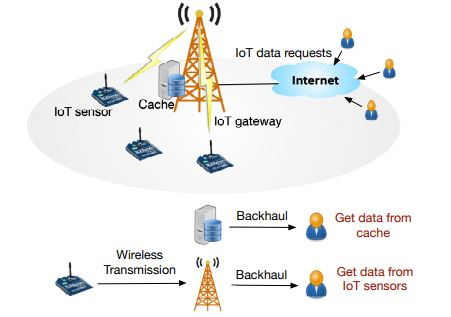
\includegraphics[width=8cm]{systemmodel}}
	\caption{نمایی از سیستم توصیف شده \cite{yao2020caching}}
	\label{fig:systemmodel}
\end{figure}

حال هرکدام از محتویات با یک شناسه‌ی یکتا\footnote{\lr{CID (Content Identifier)}} مشخص می‌گردد. در واقع در هریک از فایل‌ها، شناسه‌ی محتوا، دیتای مربوط به آن (مقدار اندازه گیری شده) به همراه دو برچسب زمانی که یکی بیانگر زمان تولید دیتا یا \lr{$t_{generation}$} و دیگری مدت زمان اعتبار مقدار اندازه‌گیری شده یا به تعبیر ریاضی \lr{$t_{life-time}$} می‌باشد. پارامتر سن دیتا نیز به صورت 
\begin{equation}\label{eq3}
	T_{life} = t_{request} - t_{generation}
\end{equation}
 تعریف می‌شود که از مقایسه‌ی آن با مدت زمان اعتبار دیتا می توان به میزان تازگی دیتا پی برد.

همانطور که پیشتر گفته شد، در هریک از گره‌های لبه یک حافظه‌ی ذخیره‌سای قرار گرفته است. برای واکشی دیتای درخواست‌های ارسالی، در صورتیکه گره لبه محتوای درخواستی را ذخیره نکرده باشد، یک درخواست به گره تولیدکننده‌ی دیتا می‌فرستد و بعد دیتای موردنظر از گره تولیدکننده واکشی می‌شود. سپس گره لبه برای ذخیره یا عدم ذخیره‌ی دیتای به دست آمده یا اینکه آیا نیاز به جایگزینی محتوا در حافظه‌ی کش وجود دارد یا نه، تصمصم می‌گیرد و دیتا را برای کاربر می‌فرستد. حال اگر دیتای درخواست شده در حافظه‌ی کش وجود داشته باشد اما تازه نباشد یا به تعبیر ریاضی \lr{$t_{age} >= t_{life}$} باشد، آنگاه گره لبه برای آپدیت دیتا به گره تولیدکننده درخواست ارسال می‌نماید و پاسخ را برای گره مصرف‌کننده نیز می‌فرستد و مقدار قبلی دیتا را با مقدار جدید جایگزین می‌نماید. حال اگر دیتای درخواست شده در حافظه‌ی کش هنوز معتبر باشد یا به تعبیر ریاضی \lr{$t_{age} < t_{life}$} باشد، آنگاه گره لبه پاسخ را برای گره مصرف‌کننده می‌فرستد و بدین صورت از ارتباط مستقیم با حسگر برای واکشی جواب جلوگیری نمودیم و بنابراین مصرف انرژی حسگر کاهش یافته و حتی نیز با میزان تأخیر کمتری دیتای درخواستی برای گره مصرف‌کننده ارسال می‌گردد. سناریوی توصیف شده را در شکل \ref{fig:simplescenario} مشاهده می‌کنید.
\begin{figure}[ht]
	\centerline{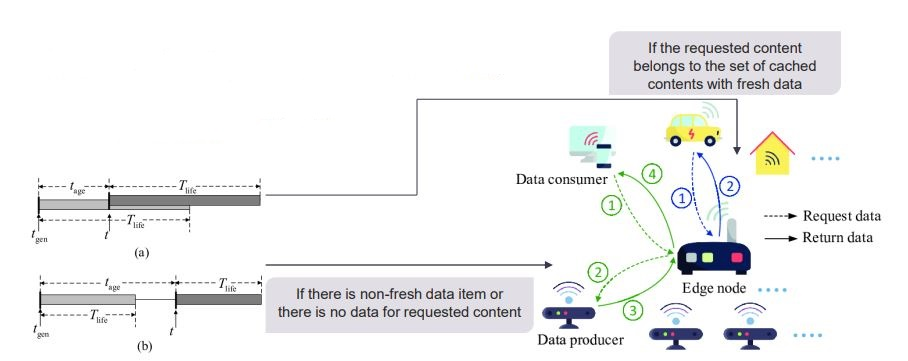
\includegraphics[width=15cm]{simplescenario}}
	\caption{سناریوی واکشی پاسخ در ذخیره‌سازی لبه برای شبکه‌های اینترنت اشیا\cite{cachingtransientdata2018}}
	\label{fig:simplescenario}
\end{figure}

\subsection{آشنایی با نمادها و ادبیات یادگیری تقویتی به کار رفته در مسئله}

\section{جمع بندی}




!
و
\verb!% !TeX root=../main.tex
\chapter{مروری بر مطالعات انجام شده}
%\thispagestyle{empty} 
\section{مقدمه}
در این فصل به مرور تعدادی از مقالات مربوط به استراتژی ذخیره‌سازی و سیاست جایگزینی محتوا در حافظه برای شبکه‌های اینترنت اشیا می‌پردازیم. در ادامه الگوریتم‌های استفاده شده در مقالات، معماری به کار رفته برای پیاده‌سازی و چالش‌های آن برای محیط  استفاده شده به طور اجمالی بیان می شوند. 

\section{مروری بر ادبیات موضوع}

\subsubsection{\lr{Caching Transient Content for IoT Sensing: Multi-Agent Soft Actor-Critic}}
	

\begin{figure}[ht]
	\centering 
	\subfloat[روش کنترلی متمرکز]{ \label{fig:centralized}
		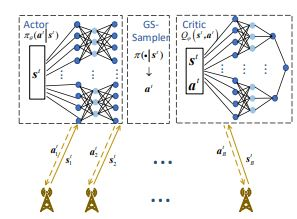
\includegraphics[width=0.4\textwidth]{centralized}}
	\hspace{2mm}
	\subfloat[روش کنترلی غیرمتمرکز]{ \label{fig:decentralized}
		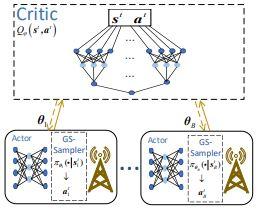
\includegraphics[width=0.4\textwidth]{decntralized}}%
	\caption{دیاگرام الگوریتم \lr{SAC} به کاررفته}
	\label{fig:centralizedvsdec} %% label for entire figure
\end{figure}

\begin{figure}[ht]
	\centerline{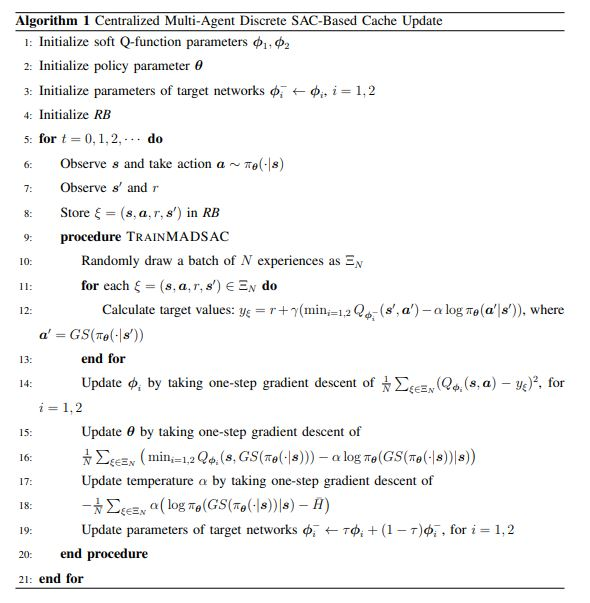
\includegraphics[width=15cm]{centralizedSAC}}
	\caption{الگوریتم \lr{Centralized Soft Actor-Critic}}
	\label{fig:cSACAlgo}
\end{figure}

\begin{figure}[ht]
	\centerline{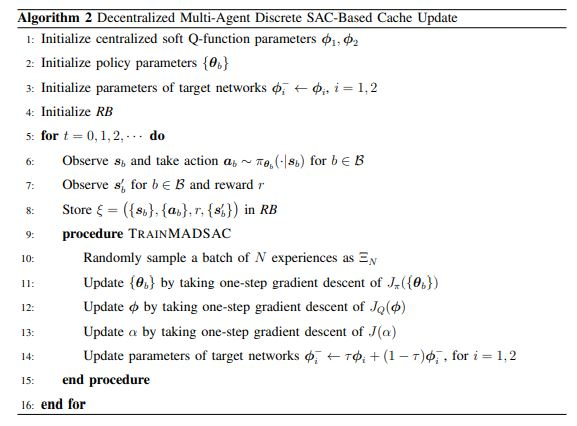
\includegraphics[width=15cm]{decentralizedSAC}}
	\caption{الگوریتم \lr{Decentralized Soft Actor-Critic}}
	\label{fig:dSACAlgo}
\end{figure}

\subsubsection{\lr{Deep Reinforcement Learning for Cooperative Content Caching in Vehicular Edge Computing and Networks}}


\begin{figure}[ht]
	\centerline{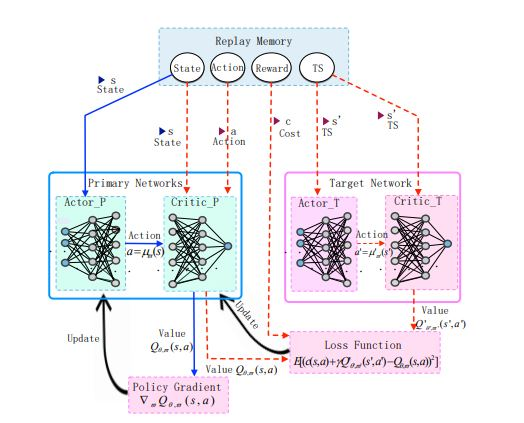
\includegraphics[width=10cm]{PG}}
	\caption{دیاگرام \lr{Deep Deterministic Policy Gradient}}
	\label{fig:PG}
\end{figure}

\begin{figure}[ht]
	\centerline{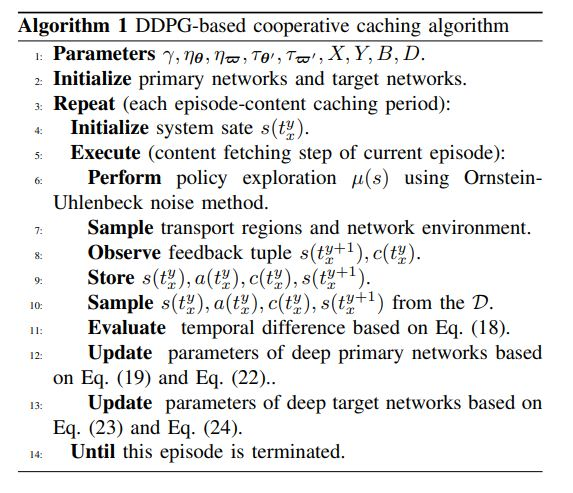
\includegraphics[width=10cm]{DDPG}}
	\caption{الگوریتم \lr{Deep Deterministic Policy Gradient}}
	\label{fig:DDPG}
\end{figure}

\subsubsection{\lr{A Deep Reinforcement Learning-Based Caching Strategy for IoT Networks with Transient Data}}


\begin{figure}[ht]
	\centerline{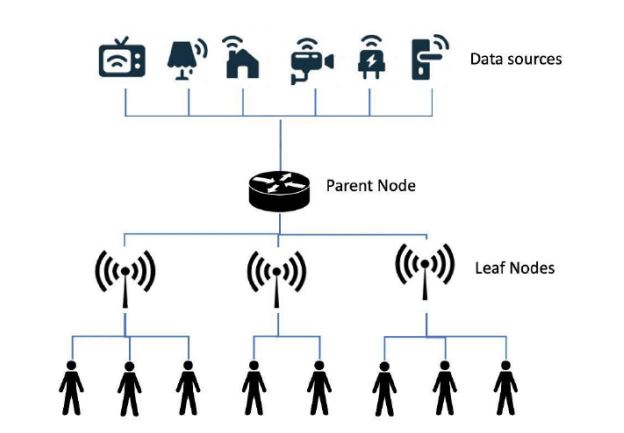
\includegraphics[width=10cm]{parent-leaf}}
	\caption{نمایی از معماری ریشه-برگ}
	\label{fig:parent-leaf}
\end{figure}

\begin{figure}[ht]
	\centerline{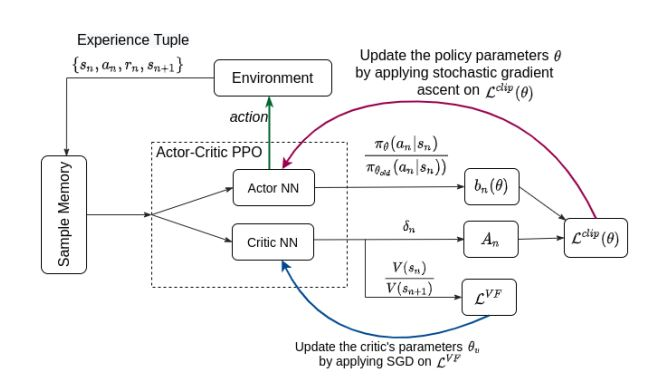
\includegraphics[width=10cm]{PPO-diagram}}
	\caption{دیاگرام \lr{Proximal Policy Optimization}}
	\label{fig:ppod}
\end{figure}

\begin{figure}[ht]
	\centerline{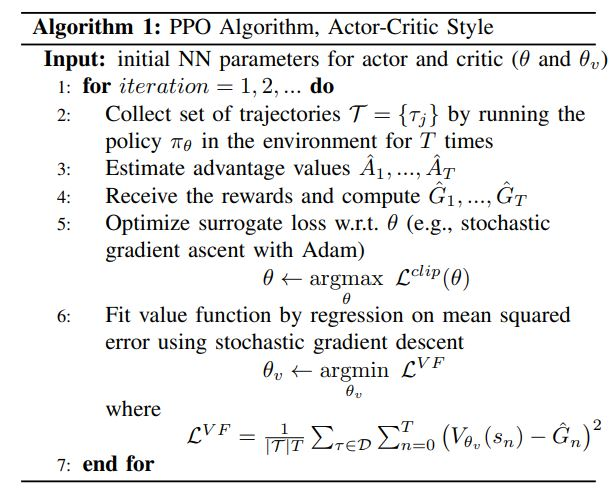
\includegraphics[width=10cm]{PPO}}
	\caption{الگوریتم \lr{Proximal Policy Optimization}}
	\label{fig:ppo}
\end{figure}

\subsubsection{\lr{HFDRL: An Intelligent Dynamic Cooperate Cashing Method Based on Hierarchical Federated Deep Reinforcement Learning in Edge-Enabled IoT}}


\begin{figure}[ht]
	\centerline{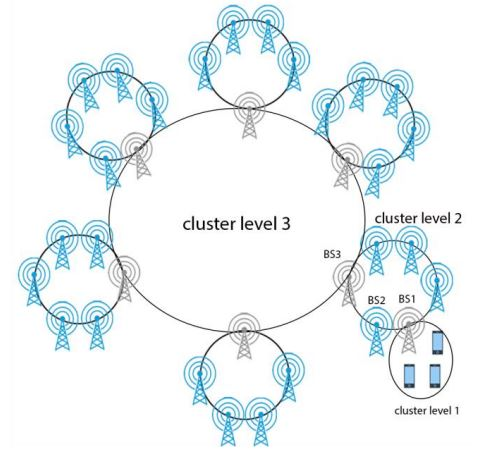
\includegraphics[width=10cm]{cluster-levels}}
	\caption{خوشه‌بندی سه‌لایه‌ای از ایستگاه‌های پایه}
	\label{fig:cluster-levels}
\end{figure}

\begin{figure}[ht]
	\centerline{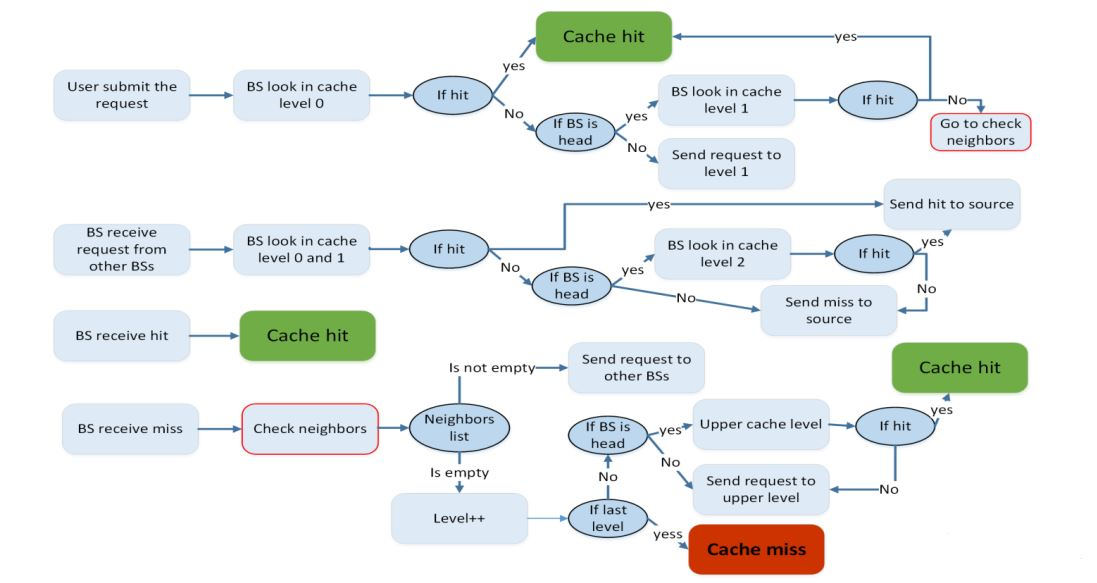
\includegraphics[width=14cm]{FDRL}}
	\caption{دیاگرام جریان داده برای پاسخ به درخواست‌های کاربران در مدل سلسله مراتبی و مشارکتی}
	\label{fig:fdrl}
\end{figure}

\begin{figure}[ht]
	\centerline{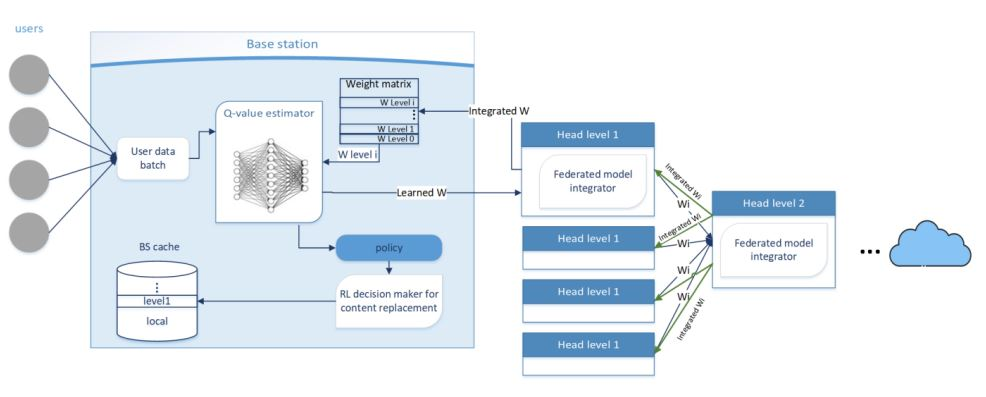
\includegraphics[width=14cm]{HFDRL}}
	\caption{مکانیزم تجمع مدل‌ها در معماری سلسله مراتبی فدراسیونی یادگیری تقویتی عمیق}
	\label{fig:hfdrl}
\end{figure}

!
را در فایل 
\lr{main.tex}،
غیرفعال%
\footnote{
برای غیرفعال کردن یک دستور، کافی است در ابتدای آن، علامت درصد انگلیسی (\%) بگذارید.
}
 کنید. در غیر این صورت، ابتدا مطالب دو فصل اول پردازش شده و سپس مطالب فصل ۳ پردازش می‌شود که این کار باعث طولانی شدن زمان پردازش می‌گردد. هر زمان که خروجی کل \پ را خواستید، تمام فصل‌ها را دوباره در
\lr{main.tex}
فعال نمائید.
بدیهتاً لازم نیست فصل‌های \پ را به ترتیب تایپ کنید. مثلاً می‌توانید ابتدا مطالب فصل ۳ را تایپ نموده و سپس مطالب فصل ۱ را تایپ کنید. 
\subsubsection{مراجع}
برای وارد کردن مراجع \پ کافی است فایل 
\lr{MyReferences.bib}
را باز کرده و مراجع خود را به شکل اقلام نمونهٔ داخل آن، وارد کنید.  سپس از \lr{bibtex} برای تولید مراجع با قالب مناسب استفاده نمائید. برای توضیحات بیشتر بخش \ref{Sec:Ref} از پیوست \ref{app:latexIntro} و نیز پیوست \ref{app:refMan} را ببینید.

\subsubsection{واژه‌نامه فارسی به انگلیسی و برعکس}
برای وارد کردن معادل فارسی اصطلاحات لاتین در متن و تهیه فهرست واژه‌نامه از آنها، از بستهٔ
\lr{glossaries}
و نرم‌افزار
\lr{xindy}
استفاده می‌شود. بدین منظور کافی است اصطلاحات لاتین و ترجمهٔ آنها را در فایل
\lr{words.tex}
وارد کرده و هر جای متن که خواستید با دستورات
\verb|gls{label}|
یا \verb|glspl{label}|
معادل فارسی مفرد یا جمع یک اصطلاح را بیاورید.

مثلا در اینجا، واژهٔ
«\gls{Action}»
برای بار اول و دوباره
«\gls{Action}»
برای بار دوم در متن ظاهر شده است.
جهت توضیحات بیشتر به پیوست
\ref{app:refMan}
مراجعه کنید.
\subsubsection{نمایه}
برای وارد کردن نمایه، باید از 
\lr{xindy}
استفاده کنید. 
%زیرا 
%\lr{MakeIndex}
%با حروف «گ»، «چ»، «پ»، «ژ» و «ک» مشکل دارد و ترتیب الفبایی این حروف را رعایت نمی‌کند. همچنین، فاصله بین هر گروه از کلمات در 
%\lr{MakeIndex}،
%به درستی رعایت نمی‌شود که باعث زشت شدن حروف‌چینی این قسمت می‌شود. 
راهنمای چگونگی کار با 
\lr{xindy} 
را می‌توانید در ویکی پارسی‌لاتک و یا مثالهای موجود در دی‌وی‌دی «مجموعه پارسی‌لاتک»، پیدا کنید.

\subsection{اگر سوالی داشتم، از کی بپرسم؟}
برای پرسیدن سوال‌های خود موقع حروف‌چینی با زی‌پرشین، می‌توانید به
\href{http://qa.parsilatex.com}{سایت پرسش و پاسخ پارسی‌لاتک}%
\LTRfootnote{http://qa.parsilatex.com}
یا
\href{http://forum.parsilatex.com}{بایگانی تالارگفتگوی قدیمی پارسی‌لاتک}%
\LTRfootnote{http://forum.parsilatex.com}
مراجعه کنید. شما هم می‌توانید روزی به سوال‌های دیگران در اینترنت جواب دهید.
بستهٔ زی‌پرشین و بسیاری از بسته‌های مرتبط با آن مانند
\lr{bidi} و
\lr{Persian-bib}،
مجموعه پارسی‌لاتک، مثالهای مختلف موجود در آن، قالب پایان‌نامه دانشگاههای مختلف و سایت پارسی‌لاتک همه به صورت داوطلبانه توسط افراد گروه پارسی‌لاتک و گروه
\lr{Persian TeX}
و بدون هیچ کمک مالی انجام شده‌اند. کار اصلی نوشتن و توسعه زی‌پرشین توسط آقای وفا خلیقی انجام شده است که این کار بزرگ را به انجام رساندند.
اگر مایل به کمک به گروه پارسی‌لاتک هستید به سایت این گروه مراجعه فرمایید:
\begin{center}
	\url{http://www.parsilatex.com}
\end{center}

\section{محتویات فصل اول یک پایان‌نامه}
فصل اول یک پایان‌نامه باید به مقدمه یا کلیات تحقیق بپردازد.
هدف از فصل مقدمه%
\LTRfootnote{Introduction}،
شرح مختصر مسأله تحقیق، اهمیت و انگیزه محقق از پرداختن به آن موضوع، بهمراه اشاره‌ای کوتاه به روش و مراحل تحقیق است. مقدمه، اولین فصل از ساختار اصلی \پ بوده و زمینه اطلاعاتی لازم را برای خواننده فراهم می‌آورد. در طول مقدمه باید سعی شود موضوع تحقیق با زبانی روشن، ساده و بطور عمیق و هدفمند به خواننده معرفی شود. این فصل باید خواننده را مجذوب و اهمیت موضوع تحقیق را آشکار سازد. در مقدمه باید با ارائهٔ سوابق، شواهد تحقیقی و اطلاعات موجود (با ذکر منبع) با روشی منظم، منطقی و هدف‌دار، خواننده را جهت داد و به سوی راه حل مورد نظر هدایت کرد. مقدمه مناسب‌ترین جا برای ارائهٔ اختصارات و بعضی توضیحات کلی است، توضیحاتی که شاید نتوان در مباحث دیگر آنها را شرح داد.

مقدمه، یکی از ارکان اساسی و اصلی پایان نامه است که مهمترین قسمت‌های آن عبارتند از: 

\subsection{عنوان تحقیق} 
باید شناختی دقیق و روشن از حوزهٔ موضوع تحقیق را عرضه دارد و خالی از هرگونه ابهام و پیچیدگی باشد.

\subsection{مسأله تحقیق}
وظیفه اصلی مقدمه بیان این مطلب به خواننده است که چرا انجام تحقیق را به عهده گرفته‌اید. اگر دلیل شما برای انجام این کار پاسخگویی به سؤال مورد علاقه‌تان است، با مشکل زیادی روبه‌رو نخواهید بود. یکی از بهترین روش‌ها برای نوشتن مقدمهٔ یک پایان‌نامه، طرح پرسش یا پرسش‌هایی مهم و اساسی است که کار تحقیقاتی شما از آغاز تا پایان قصد پاسخ دادن به آن را دارد. گاهی می‌توانید ابتدا اهمیت موضوع را بیان و سپس پرسش خود را در آن موضوع مطرح کنید.

\subsection{تاریخچه‌ای از موضوع تحقیق}
به طور کلی تشریح روندهای تحقیقاتی در محدودهٔ مورد مطالعه، مستلزم ارجاع به کارهای دیگران است. بعضی از نویسندگان برای کارهای دیگران هیچ اعتباری قائل نمی‌شوند و در مقابل، بعضی دیگر از نویسندگان در توصیف کارهای دیگران، بسیار زیاده‌روی می‌کنند. اکثر مواقع، ارجاع به مقالات دو سال قبل از کارتان، بهتر از نوشتن سطرهای مرجع است. در این قسمت باید به طور مختصر به نظرات و تحقیقات مربوط به موضوع و یا مسائل و مشکلات حل نشده در این حوزه و همچنین توجه و علاقه جامعه به این موضوع، اشاره شود.

\subsection{تعریف موضوع تحقیق}
در این قسمت محقق، موضوع مورد علاقه و یا نیاز احساس شدهٔ خود را در حوزه تحقیق بیان می‌دارد و عوامل موجود در موقعیت را تعریف و تعیین می‌کند.

\subsection{هدف یا هدف‌های کلی و آرمانی تحقیق}
این قسمت باید با جملات مثبت و کلی طرح شود و از طولانی شدن مطالب پرهیز شود.

\subsection{روش انجام تحقیق}
در این قسمت، پژوهشگر روش کاری خود را بیان می‌دارد و شیوه‌های گوناگونی را که در گردآوری مطالب خود بکار برده، ذکر می‌کند. همچنین اگر روش آماری خاصی را در تهیه و تدوین اطلاعات به کار برده است، آن شیوه را نیز اینجا بیان می‌کند.

\subsection{نوآوری، اهمیت و ارزش تحقیق}
در این قسمت، در مورد نوآوری علمی و عملی تحقیق که محقق به آن دست خواهد یافت، بحث می‌شود. ممکن است لازم باشد تا برخی نمودارهای خلاصه در این بخش استفاده شوند. به عنوان مثال، نموداری از مقاله
\cite{kim2016integrated}
در شکل
\ref{fig:sampleDiagram}
آمده است.
\begin{figure}[ht]
	\centerline{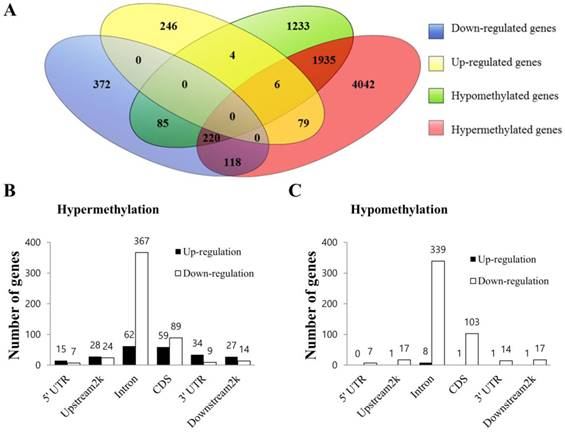
\includegraphics[width=0.8\textwidth]{journal-of-cancer_sample-result}}
	\caption{یک نمونه نمودار خلاصه برای نمایش نوآوری در نتایج
		%\cite{kim2016integrated}
	}
	\label{fig:sampleDiagram}
\end{figure}\\
طبیعتاً به صلاحدید نگارنده، شکل‌ها و نمودار‌ها می توانند در بخش های مختلف، خصوصا فصل
\ref{chap:results}
مورد استفاده قرار گیرند.

\subsection{تعریف واژه‌ها (اختیاری)}
در این قسمت محقق باید واژه‌هایی را که ممکن است برای خواننده آشنا نباشد، تعریف کند.

\subsection{خلاصه فصل‌ها}
در آخرین قسمتِ فصل اول پایان‌نامه، خلاصه‌ای اشاره‌وار از فصل‌های آتی آورده می‌شود تا خواننده بتواند تصویری واضح از دیگر قسمت‌های پایان‌نامه در ذهن خود ترسیم کند.

\section{جمع‌بندی}
در این فصل به دو مقولهٔ نحوه استفاده از قالب \پ دانشگاه تهران و نیز ویژگی‌هایی که محتویات فصل اول پایان‌نامه (یعنی مقدمه) باید داشته باشند، پرداخته شد. با توجه به اینکه این راهنما نحوه استفاده از قالب را شرح داده، ملزومات محتوایی هر فصل پایان‌نامه را توضیح می‌دهد و در پیوست‌ها نیز نحوهٔ کار با لاتک را یادآوری خواهد کرد، بنابراین مطالعهٔ کامل آن مقداری وقت شما را خواهد گرفت؛ اما مطمئن باشید از اتلاف وقت شما در ادامه کارتان تا حد زیادی جلوگیری خواهد کرد. در نوشتن متن حاضر سعی شده است علاوه بر ایجاد یک قالب لاتک برای پایان‌نامه‌های دانشگاه تهران، نکات محتوایی هر فصل نیز گوشزد گردد. طبیعتاً برای نگارش پایان‌نامهٔ خود می‌بایست مطالب تمام فصل‌ها را خودتان بازنویسی کنید.

در ادامهٔ این راهنما، تنها فصل‌هایی که یک پایان‌نامه باید داشته باشد و نیز خصوصیات یا ساختاری که محتویات هر فصل باید از آنها برخوردار باشد%
\footnote{از روی فایل «تمپلیت نگارش و تدوین پایان‌نامه \cite{UTThesisGuide}»}،
آورده می‌شوند. نهایتاً  در پیوست‌ها، مطالبی در باب یادآوری دستورات لاتک، نحوه نوشتن فرمول‌ها، تعاریف، قضایا، مثال‌ها، درج تصاویر، نمودارها، جداول و الگوریتم‌ها و نیز مدیریت مراجع، آمده است.

همچنین توصیه اکید دارم که رفع خطاهایی که احتمالاً با آنها مواجه می‌شوید را به آخر موکول نفرمایید و به محض برخورد با خطا، آن را اشکال‌زدایی و برطرف نمائید.